\documentclass[11pt]{article}
\usepackage{amsmath,amssymb,graphicx}
\usepackage{../setspace}
\addtolength{\textwidth}{1.5in}
\addtolength{\hoffset}{-1in}
\addtolength{\textheight}{1.5in}
\addtolength{\voffset}{-1in}

\title{STAT3401: Lab exercises concerning Hotelling's T$^{2}$ test}
\author{Paul Hewson}
\date{16th November 2007}
\usepackage{/usr/share/R/share/texmf/Sweave}
\begin{document}
\setlength{\parindent}{0pt}
\setlength{\parskip}{12pt}
\sffamily
\maketitle


\section{Two sampling Hotelling's T$^{2}$ test}

We are going to consider an example using data from Flea Beetles reported by Lubischew (1962) and used in Flury (1997).  We are going to use \textbf{R} as a sophisticated calculator and work through a lot of the calculations long hand first.

\begin{Schunk}
\begin{Sinput}
> library(Flury)
> ?flea.beetles
> data(flea.beetles)
\end{Sinput}
\end{Schunk}


It can be seen that there is a factor ``Species'' denoting whether the beetles are from 'oleracea' or 'carduorum'.   There are four numeric variables as follows: 'TG'; Distange of the Transverse Groove to the posterior border of
          the prothorax (microns), 'Elytra'; Length of the Elytra (in units of 0.01mm), 'Second.Antenna'; Length of the second antennal joint (microns) and 'Third.Antenna'; Length of the third antennal joint (microns).   We need to estimate the mean for each sample, and calculate the difference between the two vectors:

\begin{Schunk}
\begin{Sinput}
> mu <- by(flea.beetles[,-1], flea.beetles$Species, colMeans)
> mudiff <- mu[[1]] - mu[[2]]
> p <- dim(flea.beetles)[2] - 1 ## how many variables are we using
\end{Sinput}
\end{Schunk}

The next step is to extract the two covariance matrices:

\begin{Schunk}
\begin{Sinput}
> covmats <- by(flea.beetles[,-1], flea.beetles$Species, cov)
> covmats
\end{Sinput}
\begin{Soutput}
flea.beetles$Species: oleracea
                      TG    Elytra Second.Antenna Third.Antenna
TG             187.59649 176.86257       48.37135     113.58187
Elytra         176.86257 345.38596       75.97953     118.78070
Second.Antenna  48.37135  75.97953       66.35673      16.24269
Third.Antenna  113.58187 118.78070       16.24269     239.94152
------------------------------------------------------------ 
flea.beetles$Species: carduorum
                      TG    Elytra Second.Antenna Third.Antenna
TG             101.83947 128.06316       36.98947      32.59211
Elytra         128.06316 389.01053      165.35789      94.36842
Second.Antenna  36.98947 165.35789      167.53684      66.52632
Third.Antenna   32.59211  94.36842       66.52632     177.88158
\end{Soutput}
\end{Schunk}


and then to estimate the pooled covariance matrix $\boldsymbol{S}$ for the flea beetle data (where N[1] gives $n_{1}$,  N[2] gives $n_{2}$), can be calculated as:

\begin{Schunk}
\begin{Sinput}
> N <- xtabs(~flea.beetles[,1])
> pooledS <- ((N[1]-1) * covmats[[1]] + (N[2]-1) * covmats[[2]]) / (N[1] + N[2] -2)
> pooledS
\end{Sinput}
\begin{Soutput}
                      TG   Elytra Second.Antenna Third.Antenna
TG             143.55910 151.8034       42.52660      71.99253
Elytra         151.80341 367.7878      121.87653     106.24467
Second.Antenna  42.52660 121.8765      118.31408      42.06401
Third.Antenna   71.99253 106.2447       42.06401     208.07290
\end{Soutput}
\begin{Sinput}
> Sinv <- solve(pooledS)
> Sinv
\end{Sinput}
\begin{Soutput}
                         TG        Elytra Second.Antenna Third.Antenna
TG              0.013257964 -0.0053492256   0.0015134494 -0.0021617878
Elytra         -0.005349226  0.0066679441  -0.0047337699 -0.0005969439
Second.Antenna  0.001513449 -0.0047337699   0.0130490933 -0.0007445297
Third.Antenna  -0.002161788 -0.0005969439  -0.0007445297  0.0060093005
\end{Soutput}
\end{Schunk}


Having calculated the inverse of the pooled correlation matrix we also need the scaling factor $\frac{n_{1} n_{2}}{n_{1} + n_{2}}$.   Hotellings T$^{2}$ is then quite straightforward to calculate:


\begin{Schunk}
\begin{Sinput}
> scaleFact <- (N[1]*N[2]) / (N[1]+N[2])
> Hotellings <-  t(mudiff) %*% Sinv %*% mudiff * scaleFact
> Hotellings
\end{Sinput}
\begin{Soutput}
         [,1]
[1,] 133.4873
\end{Soutput}
\end{Schunk}


which is the value of the T$^{2}$ statistic.   We could work with this value directly, but it is more convenient to transform it into something we can compare with the $F$ distribution.

\begin{Schunk}
\begin{Soutput}
       [,1]
[1,] 30.666
\end{Soutput}
\end{Schunk}


and we compare this with an $F$ distribution having $p$ and $(n_{1} + n_{2} - p - 1)$ d.f.

And we can check this as follows:

\begin{Schunk}
\begin{Sinput}
> pf(test, p, N[1]+N[2]-p-1,lower.tail = FALSE )
\end{Sinput}
\end{Schunk}

which gives us the area under the curve from our test statistic ($30.666$) to $\infty$.   Clearly in this case, we have reject H$_{0}$, i.e. there is evidence that the mean vectors, $\bar{\boldsymbol{x}}_{oleracea} = (194.4737, 267.0526, 137.3684, 185.9474)$, $\bar{\boldsymbol{x}}_{carduorum} = (179.55, 290.80, 157.20, 209.25)$, 
 for the two species differ.   This is perhaps no surprise if you consider the data - do look at the scatterplot suggested by the helpfile.

\begin{itemize}
\item How would you modify the code to carry out a one sample T$^{2}$ test?
\item You may wish to repeat this exercise with the \texttt{turtles} data.   
\end{itemize}

You also should note that in practice this calculation is done my means of the QR decomposition, details are given in Seber (1984).   There is no in-built \textbf{R} function for doing these calculations - a nice little project for someone.   The \texttt{manova()} function can be persuaded to carry out a two sample Hotelling's T$^{2}$ test as follows:

\begin{Schunk}
\begin{Sinput}
> hotel.test <- manova(as.matrix(flea.beetles[,-1]) ~ flea.beetles[,1])
> summary(hotel.test, test = "Hotelling")
\end{Sinput}
\end{Schunk}

\section{Drawing the ellipses}


This illustration is based on, but differs from code provided by Marco Bee to accompany Flury (1997).   Firstly, we need a function to draw ellipses:

\begin{Schunk}
\begin{Sinput}
> ellipse <- function(covmat, centroid, csquare, resolution, plot = TRUE) {
+ angles <- seq(0, by = (2 * pi)/resolution, length = resolution)
+   sd <- covmat[1,2] / sqrt(covmat[1,1] * covmat[2,2])
+     projmat <- matrix(0,2,2)
+     projmat[1,1] <- sqrt(covmat[1,1] %*% (1+sd)/2)
+     projmat[1,2] <- -sqrt(covmat[1,1] %*% (1-sd)/2)
+     projmat[2,1] <- sqrt(covmat[2,2] %*% (1+sd)/2)
+     projmat[2,2] <- sqrt(covmat[2,2] %*% (1-sd)/2)
+ circle <- cbind(cos(angles), sin(angles))
+ ellipse <- t(centroid + sqrt(csquare) * projmat %*% t(circle))
+ if (plot == TRUE) {lines(ellipse)}
+ return(ellipse)
+ }
\end{Sinput}
\end{Schunk}

It is possible to define a function which calculates $c^{2}$ and calls the ellipse routine (I'm not completely convinced this is doing the calculation correctly yet, in particular I'm not sure I'm using the correct tail).

\begin{Schunk}
\begin{Sinput}
> mean.ellipse <- function (data, alpha=0.05, resolution=500) 
+ {
+ xbar <- colMeans(data)
+ n <- dim(data)[1]
+ p <- dim(data)[2]
+ f <- qf(1-alpha, p, n-p)
+ csquare <- ((n-1)/n) * (p / (n-p)) * f
+ cat(csquare) 
+ ellipse <- ellipse(cov(data), xbar, csquare, resolution)
+ }
\end{Sinput}
\end{Schunk}

%# call procedure ellips

%X <- ellips(A, m, const, k)               

%# graph the results

For illustrative purposes, we'll create a $n \times 2$ data object from our flea beetles.   Do note here that we are \emph{only} using two variables!



Given the above functions, it is quite straightforward to plot the centroids and constant density ellipses:

\begin{Schunk}
\begin{Sinput}
> X <- cbind(flea.beetles[,2], flea.beetles[,3])
> plot(X)
> points(t(colMeans(X)), pch = 16, col = "red")
> mean.ellipse(X, alpha = 0.01)
> mean.ellipse(X, alpha = 0.05)
\end{Sinput}
\end{Schunk}
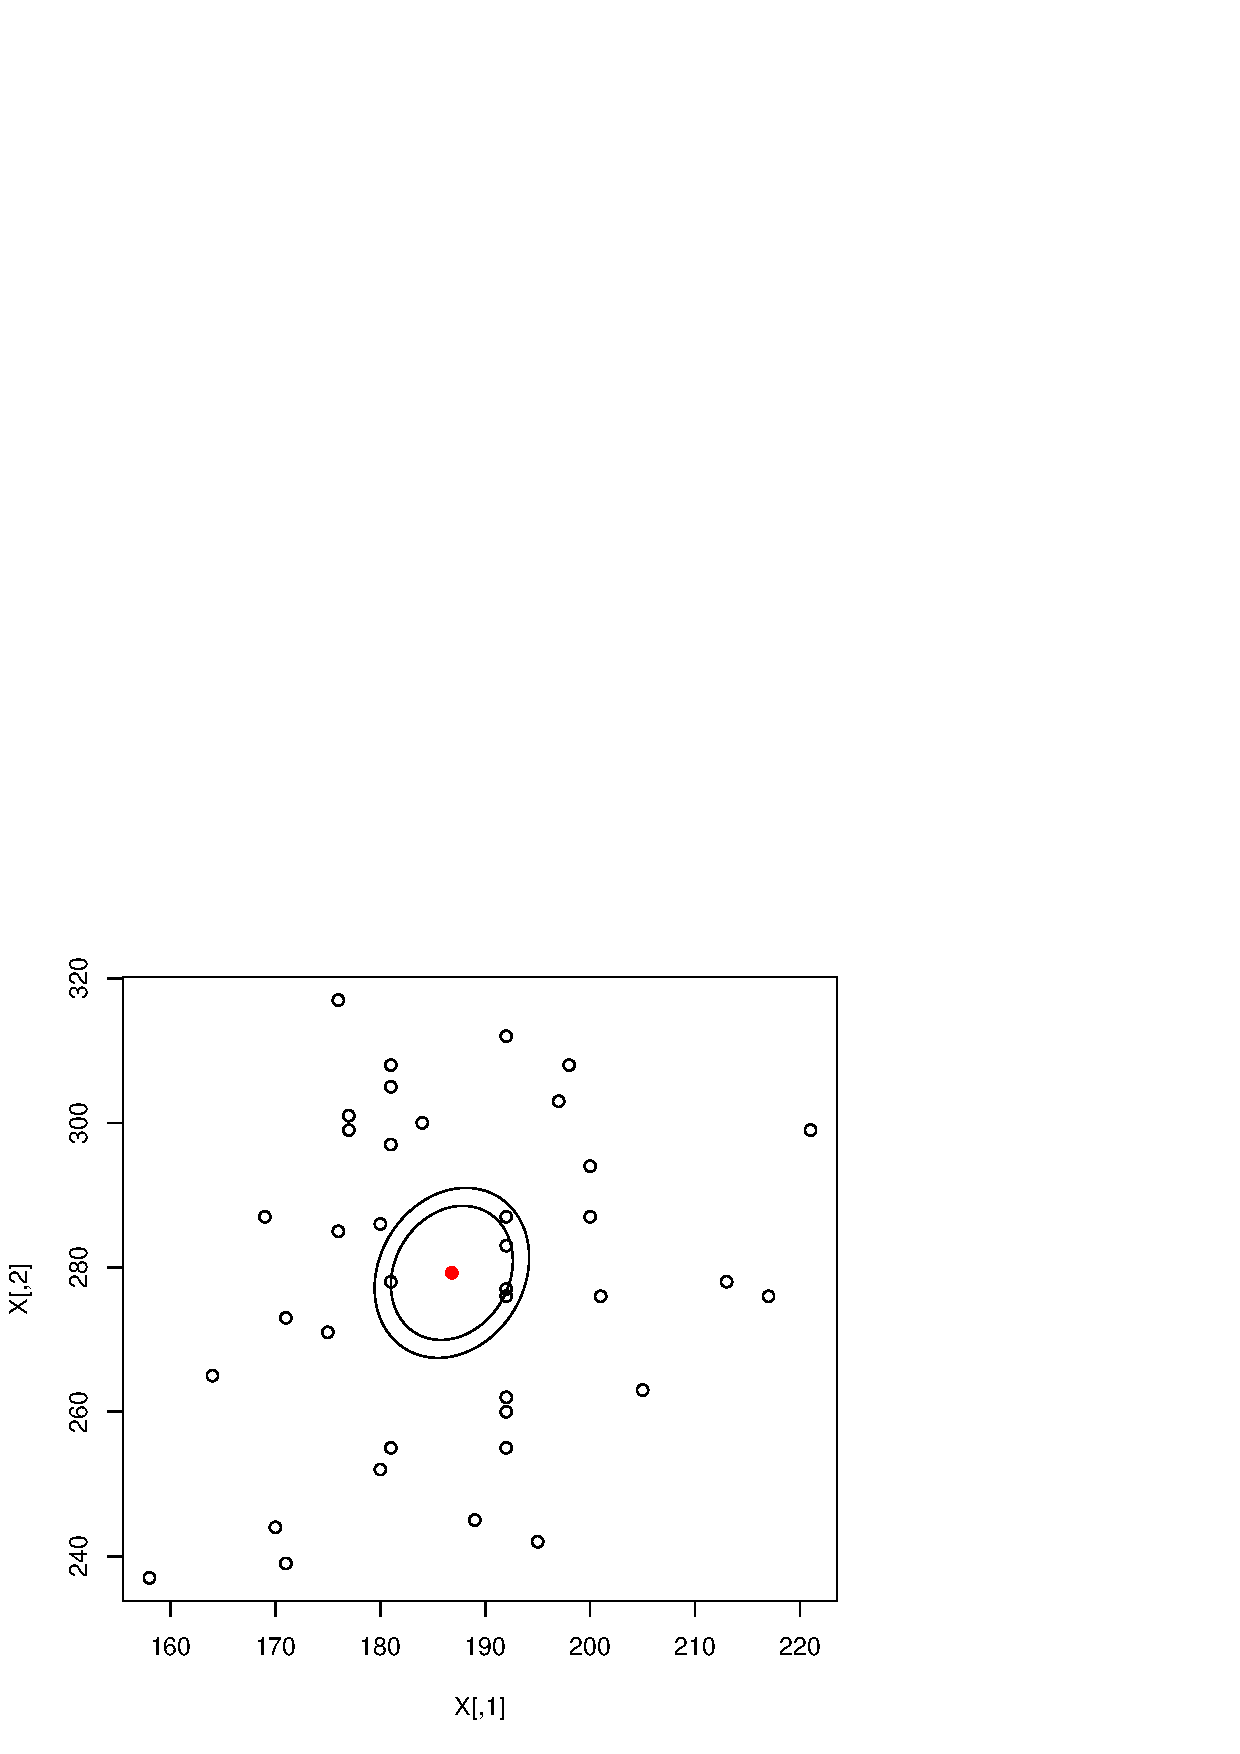
\includegraphics{STAT3401Week7HotellingLab-plotellipse}

\begin{itemize}
\item Can you estimate the elongation of the ellipse? (Well, yes you can, but how?)
\end{itemize}

You may be interested in contrasting these with the univariate confidence intervals.   As an aide memoire, some code for doing this is given below:

\begin{Schunk}
\begin{Sinput}
> abline(v = confint(lm(X[,1]~1)))
> abline(h = confint(lm(X[,2]~1)))
\end{Sinput}
\end{Schunk}

In this case you shouldn't see much difference.   But repeat this exercise withthe turtles data and you should see a very different picture.

\begin{itemize}
\item Can you plot the simultaneous confidence ellipses (see Johnson and Wichern for details)?
\end{itemize}

%X <- cbind(turtles[,2], turtles[,3])




\end{document}


